\documentclass[10pt,landscape]{article}
\usepackage{multicol}
\usepackage{calc}
\usepackage{ifthen}
\usepackage[landscape, a4paper, top=5mm, left=5mm, right=5mm, bottom=5mm]{geometry}
\usepackage[
     pdftex,
     bookmarksopen=true,
     pdfauthor={Justin Iven Müller},
     pdftitle={Lineare Algebra Cheatsheet},
     colorlinks=true,
     linkcolor=blue,
     urlcolor=blue
]{hyperref}
\usepackage{amsmath,amssymb,amsfonts}
\usepackage{enumitem}
\usepackage{tikz}
\usetikzlibrary{angles,quotes,calc}

\begin{document}
\input{content/def.tex}
\begin{multicols*}{4}

\begin{center}
     \Large{\textbf{Lineare Algebra}} \\
\end{center}

\input{content/matrixBasics.tex}
\input{content/gaussAlgorithm.tex}
\section{Vektorgeometrie}

Ein \emph{Vektor} $\vec{v}$ beschreibt eine gerichtete Translation im Raum und ist durch Richtung und Betrag $|\vec{v}|$ eindeutig bestimmt. Besondere Vektoren:
\begin{itemize}
     \item \textbf{Nullvektor} \(\vec{0}\): Ein Vektor mit Länge 0, der keine Richtung hat.
     \item \textbf{Einheitsvektor} \(\vec{e}_i\): Ein Vektor, der in der Richtung der \(i\)-ten Achse liegt und die Länge 1 hat.
     \item \textbf{Gegenvektor} \(-\vec{v}\): Ein Vektor, der die gleiche Länge wie \(\vec{v}\) hat, aber in die entgegengesetzte Richtung zeigt.
\end{itemize}


\subsection{Rechenregeln}

Vektoren lassen sich addieren und mit Skalaren $\lambda \in \mathbb{R}$ multiplizieren; beide Operationen sind komponentenweise definiert.

\textbf{Addition:}
\[
     \vec a + \vec b = \begin{pmatrix} a_1 + b_1 \\ \vdots \\ a_n + b_n \end{pmatrix}
\]

\textbf{Skalare Multiplikation}
\[
     \lambda \vec a = \begin{pmatrix} \lambda a_1 \\ \vdots \\ \lambda a_n \end{pmatrix}
\]

\subsection{Linearkombination}
Eine \emph{Linearkombination} von Vektoren $\vec a_1, \ldots, \vec a_n$ ist ein Ausdruck der Form
\[
     \vec v = \sum_{i=1}^{n} \lambda_i \vec a_i, \quad \lambda_i \in \mathbb{R}
\]

\subsection{Lineare Unabhängigkeit}
Vektoren $\vec{a}_1, \ldots, \vec{a}_n$ sind \emph{linear unabhängig}, wenn:
\[
     \vec{0} = \sum_{i=1}^{n} \lambda_i \vec{a}_i \quad \Rightarrow \quad \lambda_1 = \lambda_2 = \cdots = \lambda_n = 0
\]

\subsection{Kollinearität}
Zwei Vektoren $\vec a$ und $\vec b$ sind \emph{kollinear} (parallel), wenn einer ein Vielfaches des anderen ist:
\[
     \vec a \parallel \vec b \;\Leftrightarrow\; \exists\,\lambda\colon \vec a = \lambda\vec b
\]

\subsection{Komplanarität}
Vektoren liegen in derselben Ebene, wenn sie als Linearkombination von zwei nicht-kollinearen Vektoren dargestellt werden können:
\[
     \vec c = \lambda\vec a + \mu\vec b, \quad \text{mit } \vec a \nparallel \vec b
\]

\subsection{Koordinaten und Betrag}

Jeder Vektor im $\mathbb{R}^n$ wird durch $n$ reelle Komponenten bezüglich der Standardbasis dargestellt; sein Betrag ergibt sich aus dem Satz des Pythagoras.

\[
     \vec a = \sum_{i=1}^{n} a_i \vec e_i =
     \begin{pmatrix} a_1 \\ \vdots \\ a_n \end{pmatrix}, \qquad
     |\vec a| = \sqrt{\sum_{i=1}^{n} a_i^2}
\]
Der Verbindungsvektor von Punkt $P$ zu Punkt $Q$ und dessen Länge ist gegeben durch:
\[
     \overrightarrow{PQ} = \vec r(Q) - \vec r(P), \qquad
     \overline{PQ} = |\overrightarrow{PQ}|
\]



\subsection{Skalarprodukt}

Das \emph{Skalarprodukt} zweier Vektoren liefert eine reelle Zahl und misst den "Anteil" von $\vec{b}$ in Richtung $\vec{a}$. Es ist kommutativ und distributiv.

\[
     \vec a \cdot \vec b = \sum_{i=1}^{n} a_i b_i = |\vec a|\,|\vec b|\cos\varphi, \qquad 0 \le \varphi \le \pi
\]

\begin{center}
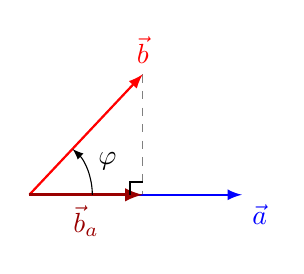
\begin{tikzpicture}[scale=0.9,>=latex]
     % vectors
     \coordinate (O) at (0,0);
     \coordinate (A) at (3,0);
     \coordinate (B) at (1.6,1.7);
     % projection of b onto a (foot point)
     \coordinate (P) at (1.6,0);

     % projection length helper line
     \draw[dashed,gray] (B) -- (P);

     % vector a
     \draw[->,thick,blue] (O) -- (A) node[below right] {$\vec a$};
     % vector b
     \draw[->,thick,red]  (O) -- (B) node[above] {$\vec b$};

     % projection b_a on a
     \draw[->,very thick,red!60!black] (O) -- (P)
          node[midway,below] {$\vec b_a$};

     % angle phi
     \pic[draw,->,"$\varphi$",angle radius=8mm,angle eccentricity=1.35]
          {angle=A--O--B};

     % right angle at foot point
     \draw (P) ++(-0.18,0) -- ++(0,0.18) -- ++(0.18,0);
\end{tikzpicture}
\end{center}

\textbf{Eigenschaften:}
\begin{itemize}
     \item Orthogonalitätstest: $\vec a \cdot \vec b = 0 \;\Leftrightarrow\; \vec a \perp \vec b$
     \item $\vec a \cdot \vec a = |\vec a|^2$
\end{itemize}


\textbf{Winkel:}
\[
     \varphi = \arccos\!\left(\frac{\vec a \cdot \vec b}{|\vec a|\,|\vec b|}\right)
\]

\textbf{Orthogonale Projektion} von $\vec b$ auf $\vec a$:
\[
     \vec b_a = \frac{\vec a \cdot \vec b}{|\vec a|^2}\,\vec a, \qquad
     |\vec b_a| = \frac{|\vec a \cdot \vec b|}{|\vec a|}
\]

\subsection{Vektorprodukt ($\mathbb{R}^3$)}

Das \emph{Vektorprodukt} zweier Vektoren im $\mathbb{R}^3$ liefert einen neuen Vektor, der senkrecht auf beiden steht. Die Richtung folgt der Rechte-Hand-Regel.

\[
     \vec a \times \vec b =
     \begin{pmatrix} a_2b_3-a_3b_2 \\ a_3b_1-a_1b_3 \\ a_1b_2-a_2b_1 \end{pmatrix}, \qquad
     |\vec a \times \vec b| = |\vec a|\,|\vec b|\sin\varphi
\]

\textbf{Eigenschaften:}
\begin{itemize}
     \item $\vec a \times \vec b \perp \vec a, \vec b$ (Richtung via Rechte-Hand-Regel)
     \item $|\vec a \times \vec b|$ = Fläche des aufgespannten Parallelogramms
     \item $\vec a \times \vec b = \vec 0 \;\Leftrightarrow\; \vec a \parallel \vec b$
     \item $\vec a \times \vec b = -(\vec b \times \vec a)$ (Antikommutativität)
     \item $\vec a \times (\vec b + \vec c) = \vec a \times \vec b + \vec a \times \vec c$ (Distributivität)
     \item $\lambda(\vec a \times \vec b) = (\lambda\vec a) \times \vec b = \vec a \times (\lambda\vec b)$ (Homogenität)
     \item $\vec e_1 \times \vec e_2 = \vec e_3$, \quad $\vec e_2 \times \vec e_3 = \vec e_1$, \quad $\vec e_3 \times \vec e_1 = \vec e_2$
\end{itemize}
\section{Geraden}

Eine \emph{Gerade} $g$ im $\mathbb{R}^n$ ist die Menge aller Punkte, die sich von einem \emph{Aufpunkt} $P$ aus in Richtung eines festen \emph{Richtungsvektors} $\vec{a} \neq \vec{0}$ erreichen lassen.

\subsection{Parameterdarstellung}
Eine Gerade $g$ lässt sich durch einen Aufpunkt $P$ und einen Richtungsvektor $\vec{a}$ mittels der folgenden Parameterdarstellung beschreiben:
\[
    g\colon \vec r(P) + \lambda \vec a, \quad \lambda \in \mathbb{R}
\]


Ein Punkt $A$ liegt auf der Geraden $g$, wenn folgendes gilt:
\[
    A \in g \;\Leftrightarrow\; \exists\,\lambda_A\colon \vec r(A) = \vec r(P) + \lambda_A \vec a
\]

\subsection{Gegenseitige Lage zweier Geraden}

Zwei Geraden im $\mathbb{R}^n$ können vier verschiedene Lagebeziehungen haben; im $\mathbb{R}^3$ kommt zusätzlich die \emph{windschiefe} Lage hinzu.

$g\colon \vec r(P) + \lambda\vec a$, \; $h\colon \vec r(Q) + \mu\vec b$:

\begin{itemize}[leftmargin=*, itemsep=0pt]
    \item $\vec a \parallel \vec b$, gemeinsamer Punkt $\Rightarrow$ \textbf{identisch}
    \item $\vec a \parallel \vec b$, kein gemeinsamer Punkt $\Rightarrow$ \textbf{echt parallel}
    \item $\vec a \nparallel \vec b$, LGS $\vec r(P)+\lambda\vec a = \vec r(Q)+\mu\vec b$ lösbar $\Rightarrow$ \textbf{schneidend}
    \item $\vec a \nparallel \vec b$, LGS unlösbar $\Rightarrow$ \textbf{windschief} (nur $\mathbb{R}^3$)
\end{itemize}

\subsection{Abstand Punkt–Gerade}

Der \emph{Abstand} eines Punktes $A$ von einer Geraden $g$ ist die Länge des kürzesten Verbindungsvektors, also die Länge des Lotes von $A$ auf $g$.

Gerade $g\colon \vec r(P) + \lambda\vec a$, Punkt $A$:

\textbf{Via Vektorprodukt} ($\mathbb{R}^3$):

\[
    l = \dfrac{|\overrightarrow{PA} \times \vec a|}{|\vec a|}
\]
\textbf{Via Projektion} ($\mathbb{R}^2$, $\mathbb{R}^3$):
\[
    l = \sqrt{|\overrightarrow{PA}|^2 - \left(\dfrac{\overrightarrow{PA}\cdot\vec a}{|\vec a|}\right)^{\!2}}
\]

\subsection{Koordinatendarstellung (nur $\mathbb{R}^2$)}
Eine Gerade $g$ im $\mathbb{R}^2$ kann auch durch eine Koordinatengleichung beschrieben werden, die einen Normalenvektor $\vec n$ enthält, der senkrecht auf der Geraden steht.
\[
    g\colon ax + by + c = 0, \qquad \vec n = \begin{pmatrix} a \\ b \end{pmatrix} \perp g
\]

\textbf{Parameter $\to$ Koordinaten:} $\lambda$ aus Komponentengleichungen eliminieren.

\textbf{Koordinaten $\to$ Parameter:} Zwei Punkte bestimmen $\to$ Aufpunkt \& Richtungsvektor.
\section{Ebenen}

Eine \emph{Ebene} $E$ im $\mathbb{R}^3$ ist die Menge aller Punkte, die sich von einem \emph{Aufpunkt} $P$ aus als Linearkombination zweier nicht-kollinearer \emph{Richtungsvektoren} $\vec{a}, \vec{b}$ erreichen lassen.

\subsection{Parameterdarstellung}
Eine Ebene $E$ lässt sich einen Aufpunkt $P$ und zwei nicht-kollineare Richtungsvektoren $\vec{a}, \vec{b}$ durch die folgende Parameterdarstellung beschreiben:
\[
     E\colon \vec{r}(P) + \lambda\vec{a} + \mu\vec{b}, \quad \lambda, \mu \in \mathbb{R}
\]

Ein Punkt $A$ liegt auf der Ebene $E$, wenn folgendes gilt:
\[
     A \in E \;\Leftrightarrow\; \exists\,\lambda_A, \mu_A\colon \vec{r}(A) = \vec{r}(P) + \lambda_A\vec{a} + \mu_A\vec{b}
\]

\subsection{Koordinatendarstellung}
Eine Ebene $E$ kann auch durch eine Koordinatengleichung beschrieben werden, die einen Normalenvektor $\vec{n}$ enthält, der senkrecht auf der Ebene steht.
\[
     E\colon ax + by + cz + d = 0, \qquad \vec{n} = \begin{pmatrix} a \\ b \\ c \end{pmatrix} \perp E
\]
Nicht eindeutig (Skalierung mit $k \neq 0$). \textbf{Normiert:} $|\vec{n}| = 1$.

\textbf{Parameter $\to$ Koordinaten:} $\vec{n} = \vec{a} \times \vec{b}$ liefert $a,b,c$; \; $d$ durch Einsetzen von $P$.

\textbf{Koordinaten $\to$ Parameter:} Drei Punkte bestimmen ($x,y$ wählen, $z$ berechnen) $\to$ Parameterdarstellung.

\subsection{Gegenseitige Lage zweier Ebenen}

Zwei Ebenen im $\mathbb{R}^3$ sind entweder identisch, echt parallel oder schneiden sich in einer Geraden. Das Kriterium hängt von der Parallelität der Normalenvektoren ab.

$E_i\colon \vec{n}_i \cdot \vec{x} + d_i = 0$ \; ($i=1,2$):
\begin{itemize}[leftmargin=*, itemsep=0pt]
     \item $\vec{n}_1 \parallel \vec{n}_2$ und $\exists\,p\neq 0\colon (a_1,b_1,c_1,d_1)=p(a_2,b_2,c_2,d_2)$ $\Rightarrow$ \textbf{identisch}
     \item $\vec{n}_1 \parallel \vec{n}_2$, nicht identisch $\Rightarrow$ \textbf{echt parallel}
     \item $\vec{n}_1 \nparallel \vec{n}_2$ $\Rightarrow$ \textbf{schneidend} (Schnittgerade via LGS, freie Variable $\to$ Parameter)
\end{itemize}

\subsection{Spezielle Lagen}

$E\colon ax+by+cz+d=0$:

\begin{center}
\small
\begin{tabular}{ll}
     \hline
     \textbf{Lage} & \textbf{Bedingung} \\
     \hline
     $\parallel$ $xy$-Ebene & $a=b=0$ \\
     $\parallel$ $xz$-Ebene & $a=c=0$ \\
     $\parallel$ $yz$-Ebene & $b=c=0$ \\
     $\parallel$ $x$-Achse  & $a=0$ \\
     $\parallel$ $y$-Achse  & $b=0$ \\
     $\parallel$ $z$-Achse  & $c=0$ \\
     \hline
\end{tabular}
\end{center}

\subsection{Abstand Punkt–Ebene}

Der \emph{Abstand} eines Punktes $A$ von einer Ebene $E$ ist die Länge des Lotes von $A$ auf $E$, gegeben durch die Hesse'sche Normalform.

Punkt $A=(x_A,y_A,z_A)$, Ebene $E\colon ax+by+cz+d=0$:
\[
     l = \frac{|ax_A + by_A + cz_A + d|}{|\vec{n}|}
\]
Normiert ($|\vec{n}|=1$): $l = |ax_A + by_A + cz_A + d|$. \quad Ursprung: $l = \frac{|d|}{|\vec{n}|}$.

\subsubsection{Schnittpunkt Ebene–Gerade}
Geradengleichung in Ebenengleichung einsetzen $\to$ Parameter $\to$ $\vec{r}(S)$.

\section{Quadratische Matrizen}

Eine Matrix $A$ heisst \emph{quadratisch}, wenn $m = n$. Die Elemente $a_{11}, a_{22}, \ldots, a_{nn}$ bilden die \emph{Hauptdiagonale}.

\subsection{Spezielle Matrizen}
\begin{itemize}
    \item \textbf{Diagonalmatrix}: Alle Elemente ausserhalb der Hauptdiagonalen $= 0$.
    \item \textbf{Einheitsmatrix} $E$: Diagonalmatrix mit allen Diagonalelementen $= 1$.
    \item \textbf{Obere Dreiecksmatrix}: $i > j \Rightarrow u_{ij} = 0$ (unterhalb $= 0$).
    \item \textbf{Untere Dreiecksmatrix}: $i < j \Rightarrow l_{ij} = 0$ (oberhalb $= 0$).
    \item \textbf{Symmetrische Matrix}: $S^T = S$.
\end{itemize}

\textbf{Einheitsmatrix:} $AE = EA = A$ \quad ($E$ spielt die Rolle der $1$).

\subsection{Potenzen}
$A^0 = E$, \quad $A^k = \underbrace{A \cdot A \cdots A}_{k}$ \quad ($k \in \mathbb{N}_{\ge 1}$)

Für Diagonalmatrizen: $D^k = \operatorname{diag}(a_{11}^k, \ldots, a_{nn}^k)$.

Im Allgemeinen: $(AB)^2 = ABAB \neq AABB = A^2B^2$ (weil Multiplikation nicht kommutativ).

\subsection{Inverse Matrizen}

Die \emph{Inverse} einer quadratischen Matrix $A$ ist $A^{-1}$ mit:
\[
    A \cdot A^{-1} = A^{-1} \cdot A = E
\]

\textbf{Inverse einer $2 \times 2$-Matrix:}
\[
    \begin{pmatrix} a & b \\ c & d \end{pmatrix}^{-1}
    = \frac{1}{ad - bc} \begin{pmatrix} d & -b \\ -c & a \end{pmatrix}
\]
Existiert nur, wenn $ad - bc \neq 0$.

\subsubsection{Invertierbar / Singulär}
\emph{Invertierbar (regulär)}: Matrix hat eine Inverse. \\
\emph{Singulär}: Matrix hat keine Inverse.

\subsubsection{Eigenschaften invertierbarer Matrizen}
\begin{enumerate}
    \item $A^{-1}$ ist eindeutig bestimmt.
    \item $(A^{-1})^{-1} = A$
    \item $(A \cdot B)^{-1} = B^{-1} \cdot A^{-1}$ \quad (Reihenfolge umkehren!)
    \item $(A^T)^{-1} = (A^{-1})^T$
\end{enumerate}

\subsubsection{Zusammenhang mit LGS}
Für $A \cdot \vec{x} = \vec{c}$ mit $n \times n$-Matrix $A$:
\[
    \vec{x} = A^{-1} \cdot \vec{c}
\]
Folgende Aussagen sind äquivalent:
\begin{enumerate}
    \item $A$ ist invertierbar
    \item $A \cdot \vec{x} = \vec{c}$ hat genau eine Lösung
    \item $\operatorname{rg}(A) = n$
\end{enumerate}

\textbf{Homogenes LGS:} $A \cdot \vec{x} = \vec{0}$. Wenn $A$ invertierbar: eindeutige Lösung $\vec{x} = \vec{0}$.

\subsubsection{Gauss-Jordan-Verfahren}
Inverse berechnen durch Zeilenumformungen:
\[
    \left( A \mid E \right) \xrightarrow{\text{Gauss-Jordan}} \left( E \mid A^{-1} \right)
\]
Falls $\operatorname{rg}(A) < n$: $A$ ist nicht invertierbar.

Diagonalmatrix: $D^{-1} = \operatorname{diag}\!\left(\frac{1}{a_{11}}, \ldots, \frac{1}{a_{nn}}\right)$, falls alle $a_{ii} \neq 0$.

\textbf{Bemerkung zum Rechnen:}
\begin{itemize}
    \item Reihenfolge beibehalten: $X \cdot A + X \cdot B = X(A+B)$, aber $\neq (A+B) \cdot X$
    \item $2X + AX \neq (2+A)X$, sondern $= (2E + A)X$
\end{itemize}

\subsection{Determinanten}

\subsubsection{2x2-Matrix}
\[
    \det\begin{pmatrix} a & b \\ c & d \end{pmatrix} = ad - bc
\]

\subsubsection{3x3-Matrix (Sarrus)}
\begin{align*}
    \det(A) = &a_{11}a_{22}a_{33} + a_{12}a_{23}a_{31} + a_{13}a_{21}a_{32}\\ 
        - &a_{13}a_{22}a_{31} - a_{11}a_{23}a_{32} - a_{12}a_{21}a_{33}
\end{align*}
Sarrus gilt \textbf{nur} für $2 \times 2$ und $3 \times 3$!

\subsubsection{Laplace-Entwicklung (\(n \times n\))}
Entwicklung nach $i$-ter Zeile:
\[
    \det(A) = \sum_{j=1}^{n} (-1)^{i+j} \cdot a_{ij} \cdot \det(A_{ij})
\]
$A_{ij}$: Matrix $A$ ohne $i$-te Zeile und $j$-te Spalte. \\
\textbf{Tipp:} Nach Zeile/Spalte mit den meisten Nullen entwickeln.

\subsubsection{Geometrische Interpretation}
\begin{itemize}
    \item $|\det(A_{2\times2})|$ = Fläche des Parallelogramms der Spaltenvektoren
    \item $|\det(A_{3\times3})|$ = Volumen des Spats der Spaltenvektoren
\end{itemize}

\subsubsection{Eigenschaften der Determinante}
\begin{enumerate}
    \item $\det(E) = 1$
    \item Dreiecksmatrix: $\det(U) = u_{11} \cdot u_{22} \cdots u_{nn}$
    \item $\det(A^T) = \det(A)$
    \item $\det(A \cdot B) = \det(A) \cdot \det(B)$
    \item $\det(A^{-1}) = \frac{1}{\det(A)}$
    \item $\det(\lambda A) = \lambda^n \cdot \det(A)$ \quad ($n \times n$-Matrix)
\end{enumerate}

\subsubsection{Äquivalenzsatz}
Für eine $n \times n$-Matrix $A$ sind äquivalent:
\begin{enumerate}
    \item $\det(A) \neq 0$
    \item Spalten von $A$ sind linear unabhängig
    \item Zeilen von $A$ sind linear unabhängig
    \item $\operatorname{rg}(A) = n$
    \item $A$ ist invertierbar
    \item $A \cdot \vec{x} = \vec{c}$ hat eine eindeutige Lösung
\end{enumerate}
\section{Vektorräume}

\subsection{Reeller Vektorraum}
Ein \emph{reeller Vektorraum} ist eine Menge $V \neq \emptyset$ mit Addition $+: V \times V \to V$ und skalarer Multiplikation $\cdot: \mathbb{R} \times V \to V$, für die gilt ($\vec{a}, \vec{b}, \vec{c} \in V$, $\lambda, \mu \in \mathbb{R}$):

\begin{enumerate}
    \item $\vec{a} + \vec{b} = \vec{b} + \vec{a}$ \quad (Kommutativ)
    \item $\vec{a} + (\vec{b} + \vec{c}) = (\vec{a} + \vec{b}) + \vec{c}$ \quad (Assoziativ)
    \item $\exists\, \vec{0} \in V: \vec{a} + \vec{0} = \vec{a}$ \quad (Neutralelement)
    \item $\forall\, \vec{a}\, \exists\, {-\vec{a}}: \vec{a} + (-\vec{a}) = \vec{0}$ \quad (Inverses)
    \item $\lambda(\mu \vec{a}) = (\lambda\mu)\vec{a}$ \quad (Assoziativ)
    \item $\lambda(\vec{a} + \vec{b}) = \lambda\vec{a} + \lambda\vec{b}$ \quad (Distributiv 1)
    \item $(\lambda + \mu)\vec{a} = \lambda\vec{a} + \mu\vec{a}$ \quad (Distributiv 2)
    \item $1 \cdot \vec{a} = \vec{a}$ \quad (Einselement)
\end{enumerate}

\textbf{Beispiele für Vektorräume:}
\begin{itemize}
    \item $\mathbb{R}^n$ (Vektoren mit $n$ Komponenten)
    \item $\mathbb{P}_n[x]$: Polynome vom Grad $\leq n$
    \item $\mathbb{R}^{m \times n}$: Menge aller $m \times n$-Matrizen
    \item $\mathbb{Z}^n/2$: Datenworte mit $n$ Bits (über Körper $\mathbb{Z}/2$)
\end{itemize}

\textbf{Kein} Vektorraum: Polynome vom Grad $= n$ (Addition kann Grad reduzieren).

\textbf{Abgeleitete Regeln:}
$0 \cdot \vec{a} = \vec{0}$, \quad $\lambda \cdot \vec{0} = \vec{0}$, \quad $(-1) \cdot \vec{a} = -\vec{a}$

\subsection{Unterräume}
Eine Teilmenge $U \subseteq V$ ist ein \emph{Unterraum} von $V$, wenn $U$ selbst ein Vektorraum ist.

\textbf{Unterraumkriterien} ($U \neq \emptyset$):
\begin{enumerate}
    \item $\vec{a}, \vec{b} \in U \Rightarrow \vec{a} + \vec{b} \in U$ \quad (abgeschlossen unter Addition)
    \item $\lambda \in \mathbb{R},\, \vec{a} \in U \Rightarrow \lambda\vec{a} \in U$ \quad (abgeschlossen unter Skalarmultiplikation)
\end{enumerate}

\textbf{Wichtig:} Falls $\vec{0} \notin U$, dann ist $U$ kein Unterraum.

\textbf{Beispiele:}
\begin{itemize}
    \item $\{\vec{0}\}$ ist immer ein Unterraum (\emph{Nullvektorraum})
    \item Geraden/Ebenen durch den Ursprung sind Unterräume von $\mathbb{R}^2$/$\mathbb{R}^3$
    \item Geraden/Ebenen \textbf{nicht} durch den Ursprung: \textbf{keine} Unterräume
    \item Symmetrische Matrizen $S^{m \times m} \subseteq \mathbb{R}^{m \times m}$: Unterraum
    \item $\mathbb{P}_2[x] \subseteq \mathbb{P}_4[x]$: Unterraum
    \item Lösungsmenge von $A\vec{x} = \vec{0}$: Unterraum von $\mathbb{R}^n$ (\emph{Kern} von $A$)
    \item Lösungsmenge von $A\vec{x} = \vec{c}$ mit $\vec{c} \neq \vec{0}$: \textbf{kein} Unterraum
\end{itemize}

\subsection{Linearer Spann}
Der lineare Spann ist die Menge aller Linearkombinationen und bildet einen Unterraum von $V$.

\[
    \operatorname{span}(\vec{b}_1, \ldots, \vec{b}_n) = \left\{ \sum_{k=1}^{n} \lambda_k \vec{b}_k \;\middle|\; \lambda_k \in \mathbb{R} \right\}
\]

\subsection{Erzeugendensystem}
$\{\vec{b}_1, \ldots, \vec{b}_n\}$ ist \emph{Erzeugendensystem} von $V$, wenn $V = \operatorname{span}(\vec{b}_1, \ldots, \vec{b}_n)$.

\textbf{Kriterium für $\mathbb{R}^m$:} Vektoren $\vec{b}_1, \ldots, \vec{b}_n \in \mathbb{R}^m$ als Spalten in $m \times n$-Matrix $B$ schreiben. Äquivalent:
\begin{enumerate}
    \item $\{\vec{b}_1, \ldots, \vec{b}_n\}$ ist Erzeugendensystem von $\mathbb{R}^m$
    \item $B \cdot \vec{x} = \vec{a}$ ist für jedes $\vec{a} \in \mathbb{R}^m$ lösbar
    \item $\operatorname{rg}(B) = m$
\end{enumerate}

\subsection{Lineare Unabhängigkeit}
$\vec{b}_1, \ldots, \vec{b}_n$ sind \emph{linear unabhängig}, wenn aus $\lambda_1 \vec{b}_1 + \ldots + \lambda_n \vec{b}_n = \vec{0}$ folgt: $\lambda_1 = \ldots = \lambda_n = 0$.

\textbf{Kriterium für $\mathbb{R}^m$:} Vektoren als Spalten in $m \times n$-Matrix $B$. Äquivalent:
\begin{enumerate}
    \item $\vec{b}_1, \ldots, \vec{b}_n$ sind linear unabhängig
    \item $B \cdot \vec{x} = \vec{0}$ hat nur die Lösung $\vec{x} = \vec{0}$
    \item $\operatorname{rg}(B) = n$
\end{enumerate}

\textbf{Zusammenhang:} Sind $\vec{b}_1, \ldots, \vec{b}_n$ linear unabhängig, so ist jede Linearkombination $\vec{a} = \lambda_1 \vec{b}_1 + \ldots + \lambda_n \vec{b}_n$ \textbf{eindeutig} (Koeffizienten eindeutig bestimmt).

\subsection{Basis und Dimension}
$\mathcal{B} = \{\vec{b}_1, \ldots, \vec{b}_n\}$ ist \emph{Basis} von $V$, wenn:
\begin{enumerate}
    \item $\mathcal{B}$ ist Erzeugendensystem von $V$
    \item $\vec{b}_1, \ldots, \vec{b}_n$ sind linear unabhängig
\end{enumerate}

\textbf{Satz für $\mathbb{R}^n$:} Vektoren $\vec{b}_1, \ldots, \vec{b}_n \in \mathbb{R}^n$ als Spalten in $n \times n$-Matrix $B$. Äquivalent:
\begin{enumerate}
    \item $\vec{b}_1, \ldots, \vec{b}_n$ bilden eine Basis von $\mathbb{R}^n$
    \item $\operatorname{rg}(B) = n$
    \item $\det(B) \neq 0$
    \item $B$ ist invertierbar
    \item $B \cdot \vec{x} = \vec{c}$ hat eine eindeutige Lösung
\end{enumerate}

Eine Basis von $\mathbb{R}^n$ besteht aus genau $n$ Vektoren. Für Erzeugendensystem braucht man $\operatorname{rg}(B) = m$, für lineare Unabhängigkeit $\operatorname{rg}(B) = n$ $\Rightarrow$ Basis erfordert $m = n$.

\textbf{Wichtige Basen:}
\begin{itemize}
    \item \emph{Standardbasis} von $\mathbb{R}^n$: $\mathcal{S} = \{\vec{e}_1, \ldots, \vec{e}_n\}$
    \item \emph{Monombasis} von $\mathbb{P}_n[x]$: $\mathcal{M} = \{1, x, x^2, \ldots, x^n\}$
\end{itemize}

\textbf{Dimension:} $\dim(V)$ = Anzahl Vekotren die eine Basis $V$ bilden.
\begin{itemize}
    \item $\dim(\mathbb{R}^n) = n$, \quad $\dim(\mathbb{P}_n[x]) = n + 1$
    \item $\dim(\mathbb{R}^{m \times n}) = m \cdot n$, \quad $\dim(S^{n \times n}) = \frac{n(n+1)}{2}$
    \item Unterraum $U \subset V$: $\dim(U) \leq \dim(V)$
    \item $\dim(\{\vec{0}\}) = 0$
\end{itemize}

\subsection{Komponentendarstellung und Basiswechsel}
Bezüglich Basis $\mathcal{B} = \{\vec{b}_1, \ldots, \vec{b}_n\}$: \quad $\vec{a} = \alpha_1 \vec{b}_1 + \ldots + \alpha_n \vec{b}_n \;\Rightarrow\; \vec{a} = \begin{pmatrix} \alpha_1 \\ \vdots \\ \alpha_n \end{pmatrix}_{\!\mathcal{B}}$

\textbf{$\mathcal{B} \to \mathcal{S}$:} Koeffizienten $\alpha_k$ und Basisvektoren $\vec{b}_k$ (in $\mathcal{S}$-Darstellung) einsetzen:
\[
    \vec{a}_{\mathcal{S}} = \alpha_1 \cdot \vec{b}_1 + \alpha_2 \cdot \vec{b}_2 + \ldots + \alpha_n \cdot \vec{b}_n = B \cdot \vec{a}_{\mathcal{B}}
\]

\textbf{$\mathcal{S} \to \mathcal{B}$:} LGS lösen: $B \cdot \vec{a}_{\mathcal{B}} = \vec{a}_{\mathcal{S}}$, wobei $B = (\vec{b}_1 \mid \vec{b}_2 \mid \ldots \mid \vec{b}_n)$.


\section{Lineare Abbildungen}

\subsection{Definition}
Eine Abbildung $f: V \to W$ zwischen zwei reellen Vektorräumen heisst \emph{linear}, wenn für alle $\vec{x}, \vec{y} \in V$ und $\lambda \in \mathbb{R}$ gilt:
\begin{enumerate}
    \item $f(\vec{x} + \vec{y}) = f(\vec{x}) + f(\vec{y})$ \quad (Additivität)
    \item $f(\lambda \cdot \vec{x}) = \lambda \cdot f(\vec{x})$ \quad (Homogenität)
\end{enumerate}
$f(\vec{x}) \in W$ heisst \emph{Bild} von $\vec{x}$.

\textbf{Nicht linear} sind z.B.: $f(x) = x + 5$, $f(x) = x^2$, $f(x) = \cos(x)$, $f(x) = e^x$.\\
Die einzigen linearen Abbildungen $\mathbb{R} \to \mathbb{R}$ sind $f(x) = m \cdot x$.

\subsection{Abbildungsmatrix (Standardbasis)}
Jede lineare Abbildung $f: \mathbb{R}^n \to \mathbb{R}^m$ lässt sich durch eine $m \times n$-Matrix $A$ darstellen:
$$f(\vec{x}) = A \cdot \vec{x}$$
Die Spalten von $A$ sind die Bilder der Standardbasisvektoren:
$$A = \begin{pmatrix} | & | & & | \\ f(\vec{e}_1) & f(\vec{e}_2) & \cdots & f(\vec{e}_n) \\ | & | & & | \end{pmatrix}$$

\subsection{Abbildungsmatrix (beliebige Basen)}
Für Vektorräume $V$ mit Basis $\mathcal{B} = \{\vec{b}_1, \ldots, \vec{b}_n\}$ und $W$ mit Basis $\mathcal{C} = \{\vec{c}_1, \ldots, \vec{c}_m\}$:
$$(f(\vec{x}))_\mathcal{C} = {}_\mathcal{C}A_\mathcal{B} \cdot \vec{x}_\mathcal{B}$$
$${}_\mathcal{C}A_\mathcal{B} = \begin{pmatrix} | & | & & | \\ (f(\vec{b}_1))_\mathcal{C} & (f(\vec{b}_2))_\mathcal{C} & \cdots & (f(\vec{b}_n))_\mathcal{C} \\ | & | & & | \end{pmatrix}$$
Die Spalten erhält man durch Lösen von LGS: $f(\vec{b}_i)$ als Linearkombination der $\vec{c}_j$ darstellen.

\subsection{Wichtige lineare Abbildungen $\mathbb{R}^2 \to \mathbb{R}^2$}

\begin{tabular}{@{}ll@{}}
\textbf{Streckung} um $\lambda_1$ in $x$, $\lambda_2$ in $y$ & $\begin{pmatrix} \lambda_1 & 0 \\ 0 & \lambda_2 \end{pmatrix}$ \\[8pt]
\textbf{Rotation} um Winkel $\varphi$ & $\begin{pmatrix} \cos\varphi & -\sin\varphi \\ \sin\varphi & \cos\varphi \end{pmatrix}$ \\[8pt]
\textbf{Spiegelung} an $x$-Achse & $\begin{pmatrix} 1 & 0 \\ 0 & -1 \end{pmatrix}$ \\[8pt]
\textbf{Spiegelung} an $y$-Achse & $\begin{pmatrix} -1 & 0 \\ 0 & 1 \end{pmatrix}$ \\[8pt]
\textbf{Punktspiegelung} am Ursprung & $\begin{pmatrix} -1 & 0 \\ 0 & -1 \end{pmatrix}$ \\[8pt]
\textbf{Scherung} in $x$-Ri.\ mit Faktor $m$ & $\begin{pmatrix} 1 & m \\ 0 & 1 \end{pmatrix}$ \\[8pt]
\textbf{Proj.\ auf} $x$-Achse & $\begin{pmatrix} 1 & 0 \\ 0 & 0 \end{pmatrix}$ \\[8pt]
\textbf{Proj.\ auf} $y$-Achse & $\begin{pmatrix} 0 & 0 \\ 0 & 1 \end{pmatrix}$
\end{tabular}

\subsection{Projektion \& Spiegelung an Gerade}
Für Gerade $g: ax + by = 0$ mit $a^2 + b^2 = 1$ (normiert!):

\textbf{Orthogonale Projektion:}
$P = \begin{pmatrix} 1-a^2 & -ab \\ -ab & 1-b^2 \end{pmatrix}$, \quad $p(\vec{x}) = \vec{x} - (\vec{n} \cdot \vec{x}) \cdot \vec{n}$

\textbf{Spiegelung:}
$S = \begin{pmatrix} 1-2a^2 & -2ab \\ -2ab & 1-2b^2 \end{pmatrix}$, \quad $s(\vec{x}) = \vec{x} - 2(\vec{n} \cdot \vec{x}) \cdot \vec{n}$

Dabei ist $\vec{n} = \binom{a}{b}$ der normierte Normalenvektor.

\vfill

\rule{0.3\linewidth}{0.25pt}
\scriptsize

By Justin Iven Müller (2026)
\href{https://github.com/JustinIven/zhaw-cheatsheets}{github.com/JustinIven/zhaw-cheatsheets}


\end{multicols*}
\end{document}
